\begin{enumerate}[label=\thesubsection.\arabic*.,ref=\thesubsection.\theenumi]

\item
 The open-loop transfer function of a plant in a unity feedback configuration is given as 
\begin{align}
    G\brak{s} &= \frac{K(s+4)}{(s+8)(s^{2}-9)}
\end{align}
Find  the value of the gain $K>0$ for which $-1 + \j2$ lies on the root locus.
%
\\
\solution
  The closed loop transfer function for a negative feed back system is:
  \begin{align}
      F\brak{s} &= \frac{G\brak{s}}{1+G\brak{s}H\brak{s}}
  \end{align}
%
From the characteristic equation
Since it is a unity feed back system, $H\brak{s} = 1$, and now using the characteristic align at $s_{1} = -1 + \j2$

\begin{align}
    1 + G\brak{s_{1}}H\brak{s_{1}} &= 0 
\\
\implies    \abs{G\brak{s_{1}}} &= \frac{K\sqrt{13}}{\sqrt{51}\sqrt{8}\sqrt{20}} = 1 
\\
\implies     K &= 25.05
\\
\text{or, }    F\brak{s} &= \frac{25.05(s+4)}{s^{3}+8s^{2}+16.05s+28.2} 
\end{align}
%
The following code plots the root locus in Fig. \ref{fig:ee18btech11052}.
%
\begin{figure}
\centering
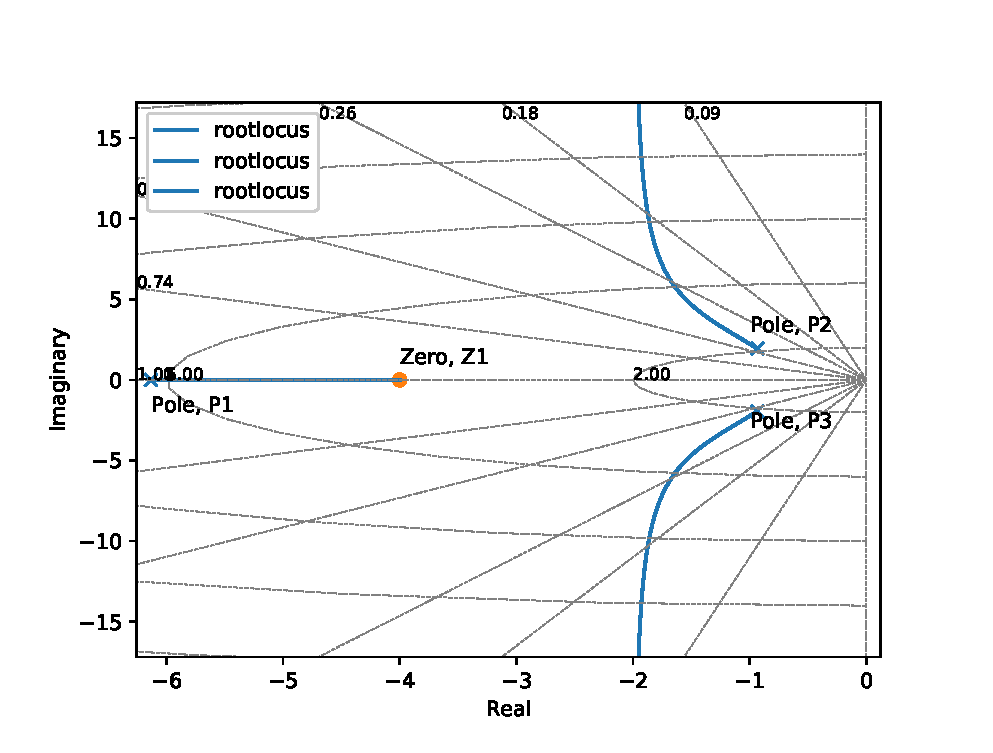
\includegraphics[width =\columnwidth]{./figs/ee18btech11052.eps}
\caption{}
\label{fig:ee18btech11052}
\end{figure}


\begin{lstlisting}
codes/ee18btech11052.py
\end{lstlisting}
    
\end{enumerate}

